\documentclass[openany,12pt,UTF8]{ctexart}
\usepackage[a4paper,margin=2.5cm]{geometry}
\usepackage{amsmath}                                    % 排版数学公式

% 使equation计数器也依赖于section计数器
\numberwithin{equation}{section}

% 使table计数器也依赖于section计数器
\numberwithin{table}{section}

% 使figure计数器也依赖于section计数器
\numberwithin{figure}{section}

\usepackage{latexsym}
\usepackage{amsfonts}                                   %数学符号字体库宏包套件,它包含有:amsfonts、amssymb、eufrak 和 eucal 四个宏包。
\usepackage{amssymb}                                    % 定义AMS的数学符号命令
\usepackage{mathrsfs}                                   % 数学RSFS书写字体
\usepackage{bm}                                         % 数学黑体
\usepackage{graphicx}                                   % 支持插图,图形宏包graphics的扩展宏包
\usepackage{color,xcolor}                               % 支持彩色
\usepackage{amscd}
\usepackage[linesnumbered,ruled,vlined]{algorithm2e}
\usepackage{diagbox}
\usepackage{minted}
\usepackage{titlesec}                                   %设置章节格式
\usepackage{tcolorbox}

% 设置 paragraph 为只有一级编号(从1开始)
\renewcommand{\theparagraph}{\arabic{paragraph}} % 只显示一级编号
\makeatletter
\@addtoreset{paragraph}{section} % 每节开始时重置 paragraph 计数器
\makeatother

%%文本框设置
\newcommand{\tbox}[1]{
  \begin{center}
    \begin{tcolorbox}[colback=gray!10,%gray background
        colframe=black,% black frame colour
        width=14cm,% Use 8cm total width,
        arc=1mm, auto outer arc,
        boxrule=0.5pt,
      ]
      {#1}
    \end{tcolorbox}
  \end{center}
}

% 设置 paragraph 为 block 风格,自动换行
\titleformat{\paragraph}[block]
  {\normalfont\normalsize\bfseries}{\theparagraph.}{0.5em}{}

% 设置标题后换行(after-sep 设为 \newline)
\titlespacing*{\paragraph}{0pt}{3.25ex plus 1ex minus .2ex}{0pt}
  
\usepackage{enumerate}                                 	%更改enumerate环境格式
\usepackage{hyperref}

%改变超链接颜色
\hypersetup{
    colorlinks=true,
    linkcolor=blue,
    filecolor=blue,      
    urlcolor=blue,
    citecolor=cyan,
}

\usepackage{subcaption}
\usepackage{minipage-marginpar}
\usepackage{float}%提供float浮动环境
\usepackage{booktabs}%提供命令\toprule、\midrule、\bottomrule
\usepackage{listings}
\usepackage{xcolor}
\usepackage{tabularx}
\usepackage{multirow}
\usepackage[perpage]{footmisc}

% 自定义命令,用于角标引用文献和交叉引用
\newcommand{\scite}[1]{\textsuperscript{\cite{#1}}}
\newcommand{\sref}[1]{\textsuperscript{\ref{#1}}}
\newcommand{\bs}[1]{\boldsymbol{#1}}
\newcommand{\romannumber}[1]{\uppercase\expandafter{\romannumeral#1}}
\newcommand{\alert}[1]{\textcolor{red}{#1}}
%%对一些autoref的中文引用名作修改
\def\equationautorefname{式}
\def\footnoteautorefname{脚注}
\def\itemautorefname{项}
\def\figureautorefname{图}
\def\tableautorefname{表}
\def\partautorefname{篇}
\def\appendixautorefname{附录}
\def\chapterautorefname{章}
\def\sectionautorefname{节}
\def\subsectionautorefname{小小节}
\def\subsubsectionautorefname{subsubsection}
\def\paragraphautorefname{段落}
\def\subparagraphautorefname{子段落}
\def\FancyVerbLineautorefname{行}
\def\theoremautorefname{定理}

% 设置标题层级和目录层级
\setcounter{tocdepth}{3}
\setcounter{secnumdepth}{4}
\usepackage{rotating}
\title{程序说明}
\author{欧阳嘉鸿}
\date{\today}
\begin{document}
\maketitle
\newpage
\tableofcontents
\newpage
\section{探测任务规划问题建模}

\subsection{数据结构与符号说明}
在本模型中,主要涉及的集合、参数和变量如\autoref{table:主要数据结构与符号说明}所示。其中,弧段集合 $A_{r,s}$ 的生成依赖于观测窗口字典 \texttt{radar\_target\_vis\_dict}。该字典的键为测站-目标编号对 $(r,s)$,值为该测站可观测该目标的多个时间窗口,每个时间窗口用一个三元组 $(t_{\text{start}}, t_{\text{end}}, \Delta t)$ 表示,分别对应仿真起止时间点的索引与持续时长(分钟)。该结构最初由可见性分析模块根据轨道仿真生成,并经由 MATLAB 的 \texttt{usableArcs.mat} 文件导入。

变量 \texttt{x[r][s][a]} 为核心的布尔决策变量,用于表示是否选择雷达 $r$ 在第 $a$ 个弧段上观测目标 $s$。该变量由 COPT 求解器在建模阶段创建,在求解后可通过 \texttt{x[r][s][a].x} 获取其值(0 或 1)。变量 \texttt{y[s]} 表示目标 $s$ 是否被有效观测(即满足其所有观测需求约束),是模型中用于综合评估任务完成情况的辅助变量。

输入数据结构中,\texttt{sensor\_data} 与 \texttt{require\_data} 分别来自 Excel 文件 \texttt{sensorData.xlsx} 和 \texttt{requireData.xlsx},字段对应关系如\autoref{tab:data-fields}所示。
\begin{table}[H]
    \centering
    \caption{输入数据字段与模型变量的对应关系}
    \label{tab:data-fields}
    \begin{tabular}{lll}
        \toprule
        \textbf{数据字段来源}        & \textbf{字段名称}            & \textbf{模型中对应符号}      \\
        \midrule
        \texttt{sensor\_data}  & \texttt{雷达编号}            & 构建雷达集合 $R$            \\
                               & \texttt{最大探测目标数}         & 各雷达最大观测能力 $C_r$       \\
        \addlinespace
        \texttt{require\_data} & \texttt{目标编号}            & 构建目标集合 $S$            \\
                               & \texttt{需要的测站数量}         & 最小观测测站数 $M_s^{\min}$  \\
                               & \texttt{需要的弧段数量}         & 最小观测弧段数 $N_s^{\min}$  \\
                               & \texttt{需要的观测时间(min)}    & 最小累计观测时长 $T_s^{\min}$ \\
                               & \texttt{优先级(数值越大,优先级越高)} & 优先级权重 $w_s$           \\
        \bottomrule
    \end{tabular}
\end{table}

程序通过读取测站参数表 \texttt{sensorData.xlsx} 生成数据框 \texttt{sensor\_data},其中字段 \texttt{sensor\_data["雷达编号"]} 提供每个测站的唯一标识,用于构建雷达集合 $R$;字段 \texttt{sensor\_data["最大探测目标数"]} 表示每个测站在任一时刻最多可同时观测的目标数,对应模型中的参数 $C_r$。任务需求表 \texttt{requireData.xlsx} 被加载为数据框 \texttt{require\_data},记录每一个观测目标的基本属性及其观测需求:\texttt{require\_data["目标编号"]} 用于构建目标集合 $S$;\texttt{require\_data["需要的测站数量"]} 表示每个目标所需的最小观测测站数,记作 $M_s^{\min}$;\texttt{require\_data["需要的弧段数量"]} 表示所需的最小观测次数,记作 $N_s^{\min}$;\texttt{require\_data["需要的观测时间(min)"]} 是累计观测时长的最小值(单位为分钟),映射为 $T_s^{\min}$;而 \texttt{require\_data["优先级(数值越大,优先级越高)"]} 表示任务重要性,用于构建目标函数中的权重系数 $w_s$。

此外,时间节点矩阵 \texttt{simDate} 是一个二维数组,表示整个仿真周期内的统一时间参考,供弧段时间索引定位与可视化模块使用。仿真起始时间 \texttt{start\_time} 用于构造 UTC 时间标签。通过模型求解后,遍历所有 \texttt{x[r][s][a]} 的值即可输出完整的调度方案,包括观测起止时间与分配的测站资源,适用于后续的任务下发与动态更新。

\subsection{数学模型}
本问题旨在为多个地面雷达调度多个空间目标的观测任务,实现有效资源分配并最大化任务完成度。
\subsubsection{决策变量}
定义如下布尔型决策变量:
$$
    x_{r,s,a} =
    \begin{cases}
        1, & \text{若雷达 } r \text{ 在其第 } a \text{ 个可见弧段对目标 } s \text{ 进行观测} \\
        0, & \text{否则}
    \end{cases}
$$
其中:$r \in R$(雷达集合),$s \in S$(目标集合),$a \in A_{r,s}$(雷达 $r$ 对目标 $s$ 可观测的弧段索引集合)

\subsubsection{目标函数}
\tbox{
首先,我们定义以下两个关键概念:

\textbf{有效观测}:若雷达 $r$ 对目标 $s$ 的一次观测满足观测时长 $t_{r,s}$ 大于目标要求的最小观测时长 $T_s^{\min}$,则称这次观测为有效观测。

\textbf{有效观测目标}:若目标 $s$ 从 $N_r$ 个不同雷达处共获得 $N_s$ 次有效观测,并且 $N_r$ 不小于目标要求的最小测站数量 $M_s^{\min}$,且 $N_s$ 不小于目标要求的最小有效观测次数 $N_s^{\min}$,则称目标 $s$ 为有效观测目标。
}

目标函数采用两阶段建模方式,第一阶段最大化加权有效观测目标数,第二阶段在保证主目标不变的前提下最小化雷达观测弧段总数:

\paragraph{第一阶段目标函数:}
$$
    \max J_1 = \sum_{s \in S} w_s \cdot y_s
$$
其中:
\begin{itemize}
    \item $w_s$:目标 $s$ 的权重(优先级);
    \item $y_s$:二值变量,表示目标 $s$ 是否为有效观测目标。
\end{itemize}

\paragraph{第二阶段目标函数:}
$$
    \min J_2 = \sum_{r \in R}\sum_{s \in S}\sum_{a \in A_{r,s}} x_{r,s,a}
$$

该两阶段目标函数设计确保了模型在优先保障高权重目标的前提下,尽可能节省雷达资源,提高系统整体效率。

\subsubsection{约束条件}

\paragraph{雷达观测容量约束}\

每部雷达在任一时刻最多只能同时观测 $C_r$ 个目标。考虑离散时间索引 $t \in T$,有:
$$
    \sum_{s \in S} \sum_{a \in A_{r,s}^t} x_{r,s,a} \leq C_r, \quad \forall r \in R,\ \forall t \in T
$$
其中:
\begin{itemize}
    \item $A_{r,s}^t$:时刻 $t$ 时,雷达 $r$ 可用于观测目标 $s$ 的弧段集合
    \item $T$:时间步长集合
\end{itemize}

\paragraph{目标有效性判定约束(逻辑约束)}\

利用中间变量辅助建模,通过观测决策 $x_{r,s,a}$ 与弧段持续时间 $t_{r,s,a}$ 的乘积累加可得目标有效观测时长,再结合目标对观测数量和测站的要求,判定 $y_s$。

以上构成了完整的多雷达-多目标探测任务规划模型。

\section{探测任务规划方法说明}
\subsection{使用的求解器}
本项目使用杉数科技提供的商业混合整数规划求解器 COPT(Cardinal Optimizer)。该求解器支持高性能求解大规模 MILP、MIQP 等优化问题,并支持 Python 接口与 Gurobi 接近。具体使用过程中,通过构建 COPT 模型对象、添加变量与约束、设置目标函数并调用 \texttt{model.solve()} 进行求解。

\subsection{规划方法的基本原理}
我们采用标准的混合整数规划方法对问题建模求解。初始时,程序从观测窗口表中构建弧段数据,并根据任务参数构建布尔决策变量。每轮迭代中,求解器根据目标函数最大化原则动态调整变量组合,直至收敛或达到终止条件。由于初期目标函数值往往较低,求解器通过迭代优化调度方案,逐步提升有效观测数量,提升资源利用率。

在建模过程中,我们引入了两阶段目标函数设计,先最大化加权有效观测目标数,然后在此基础上最小化总的雷达观测弧段数量。这种策略不仅提升了模型的求解效率,也增强了调度方案的可行性与鲁棒性。

\section{探测任务方案生成结果}
\subsection{仿真参数}
在本次仿真实验中,我们选择了 193 颗星链卫星以及 40 部地面雷达(包含精密跟踪雷达和相控阵雷达)进行调度仿真。具体参数如\autoref{table:仿真参数设置}所示。
\begin{table}[h]
    \centering
    \caption{仿真参数设置}
    \label{table:仿真参数设置}
    \begin{tabular}{>{$}l<{$} | l | l}
        \hline
        \textbf{参数名称}  & \textbf{说明} & \textbf{数值}                    \\
        \hline
        \Delta t       & 时间步长        & 1\,\text{min}                  \\
        T_{\text{sim}} & 仿真总时长       & 1440\,\text{min}(1天)           \\
        T_s^{\min}     & 各目标最小观测时长   & 3\,\text{min} -- 6\,\text{min} \\
        M_s^{\min}     & 各目标所需最小测站数量 & 2 -- 3                         \\
        N_s^{\min}     & 各目标最小有效观测次数 & 4 -- 6                         \\
        C_r            & 各雷达的同时观测容量  & 1(精密跟踪)或 80(相控阵)               \\
        \hline
    \end{tabular}
\end{table}

\subsection{探测任务方案结果}
在进行混合整数规划求解后,获得了一组可行的观测任务分配方案。\autoref{tab:schedule_summary}是其中部分雷达-目标观测计划摘要(表格仅展示一部分结果)。

此外,我们运用HTML的形式,能够选择想要展示的方式,展示任务分配表格和任务甘特图。单个测站的甘特图如\autoref{figure:102测站分配的任务甘特图}所示。
单个目标被分配的观测任务如\autoref{figure:63411目标被分配的任务甘特图}所示。HTML网页操作界面如\autoref{figure:网页界面示意}所示。
\begin{figure}[h]\centering
    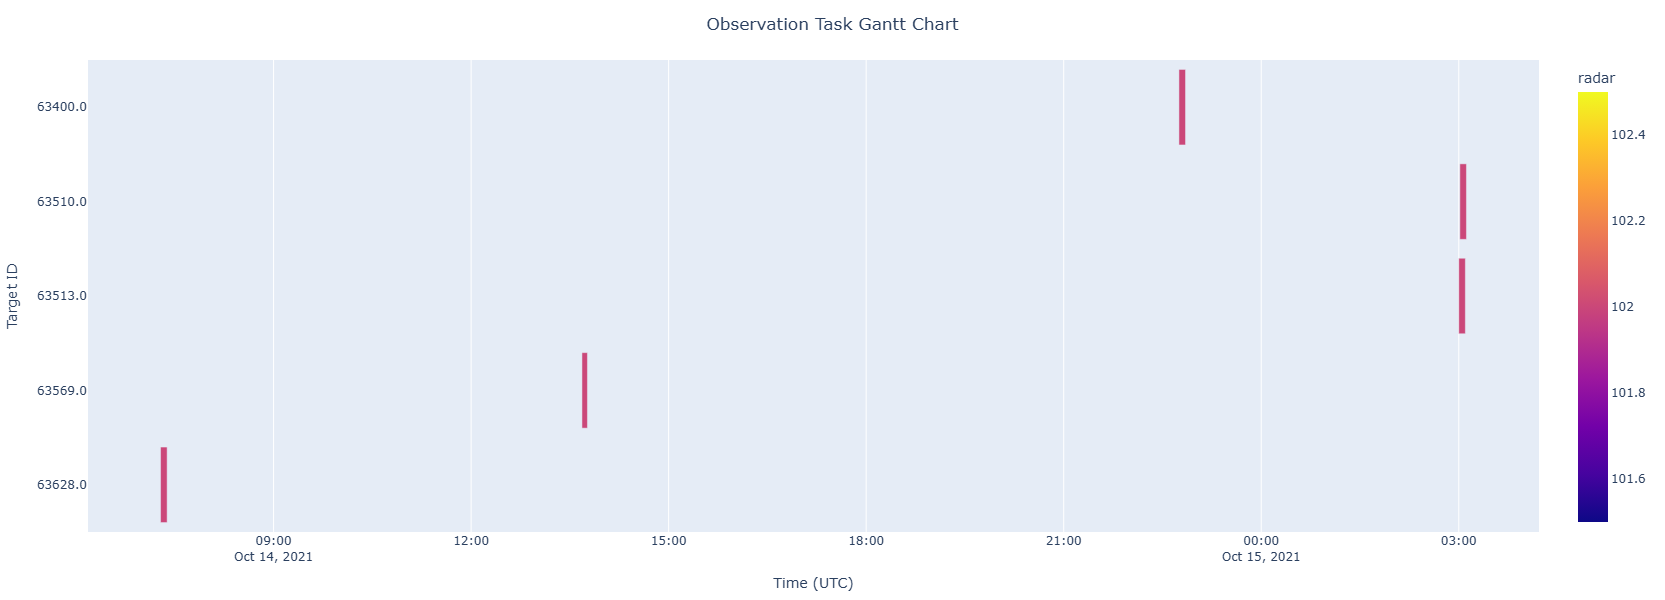
\includegraphics[width=\columnwidth]{figures/102测站.png}
    \caption{102测站分配的任务甘特图}
    \label{figure:102测站分配的任务甘特图}
\end{figure}
\begin{figure}[h]\centering
    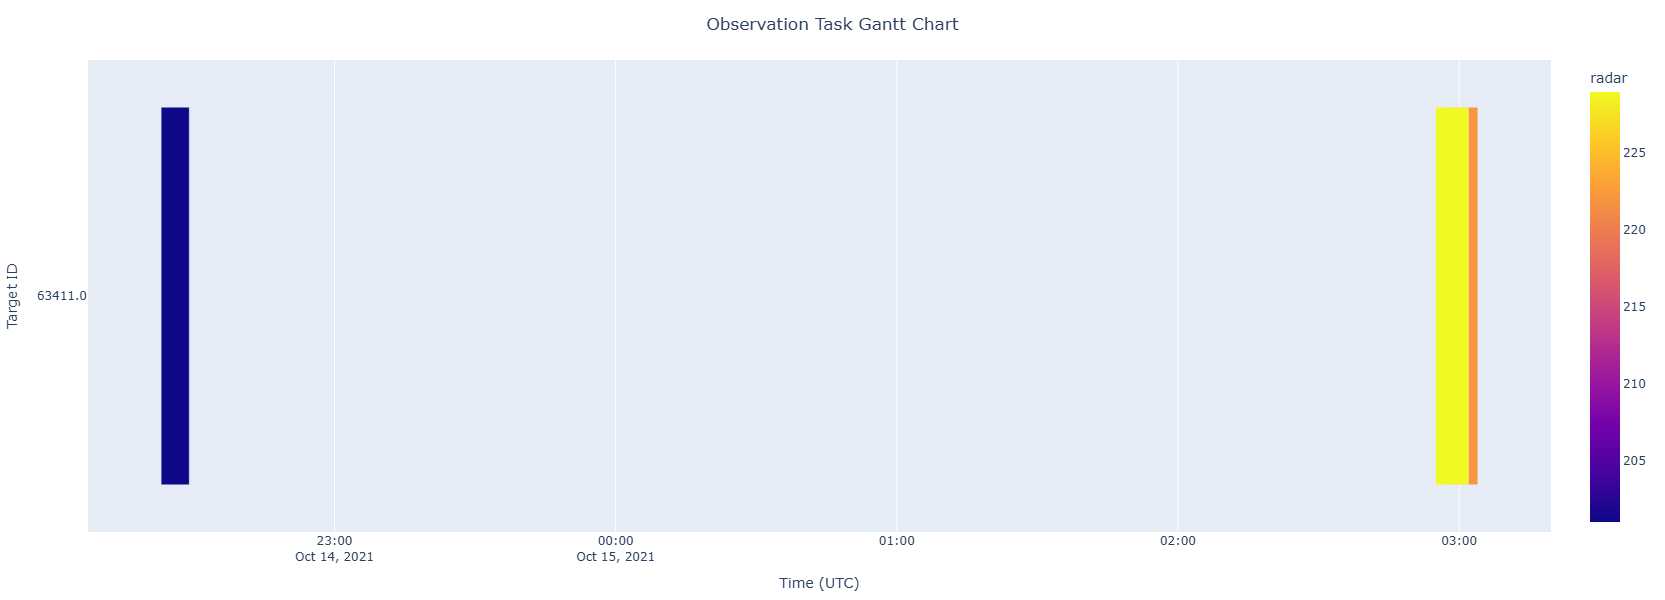
\includegraphics[width=\columnwidth]{figures/63411目标.png}
    \caption{63411目标被分配的任务甘特图}
    \label{figure:63411目标被分配的任务甘特图}
\end{figure}
\begin{figure}[h]\centering
    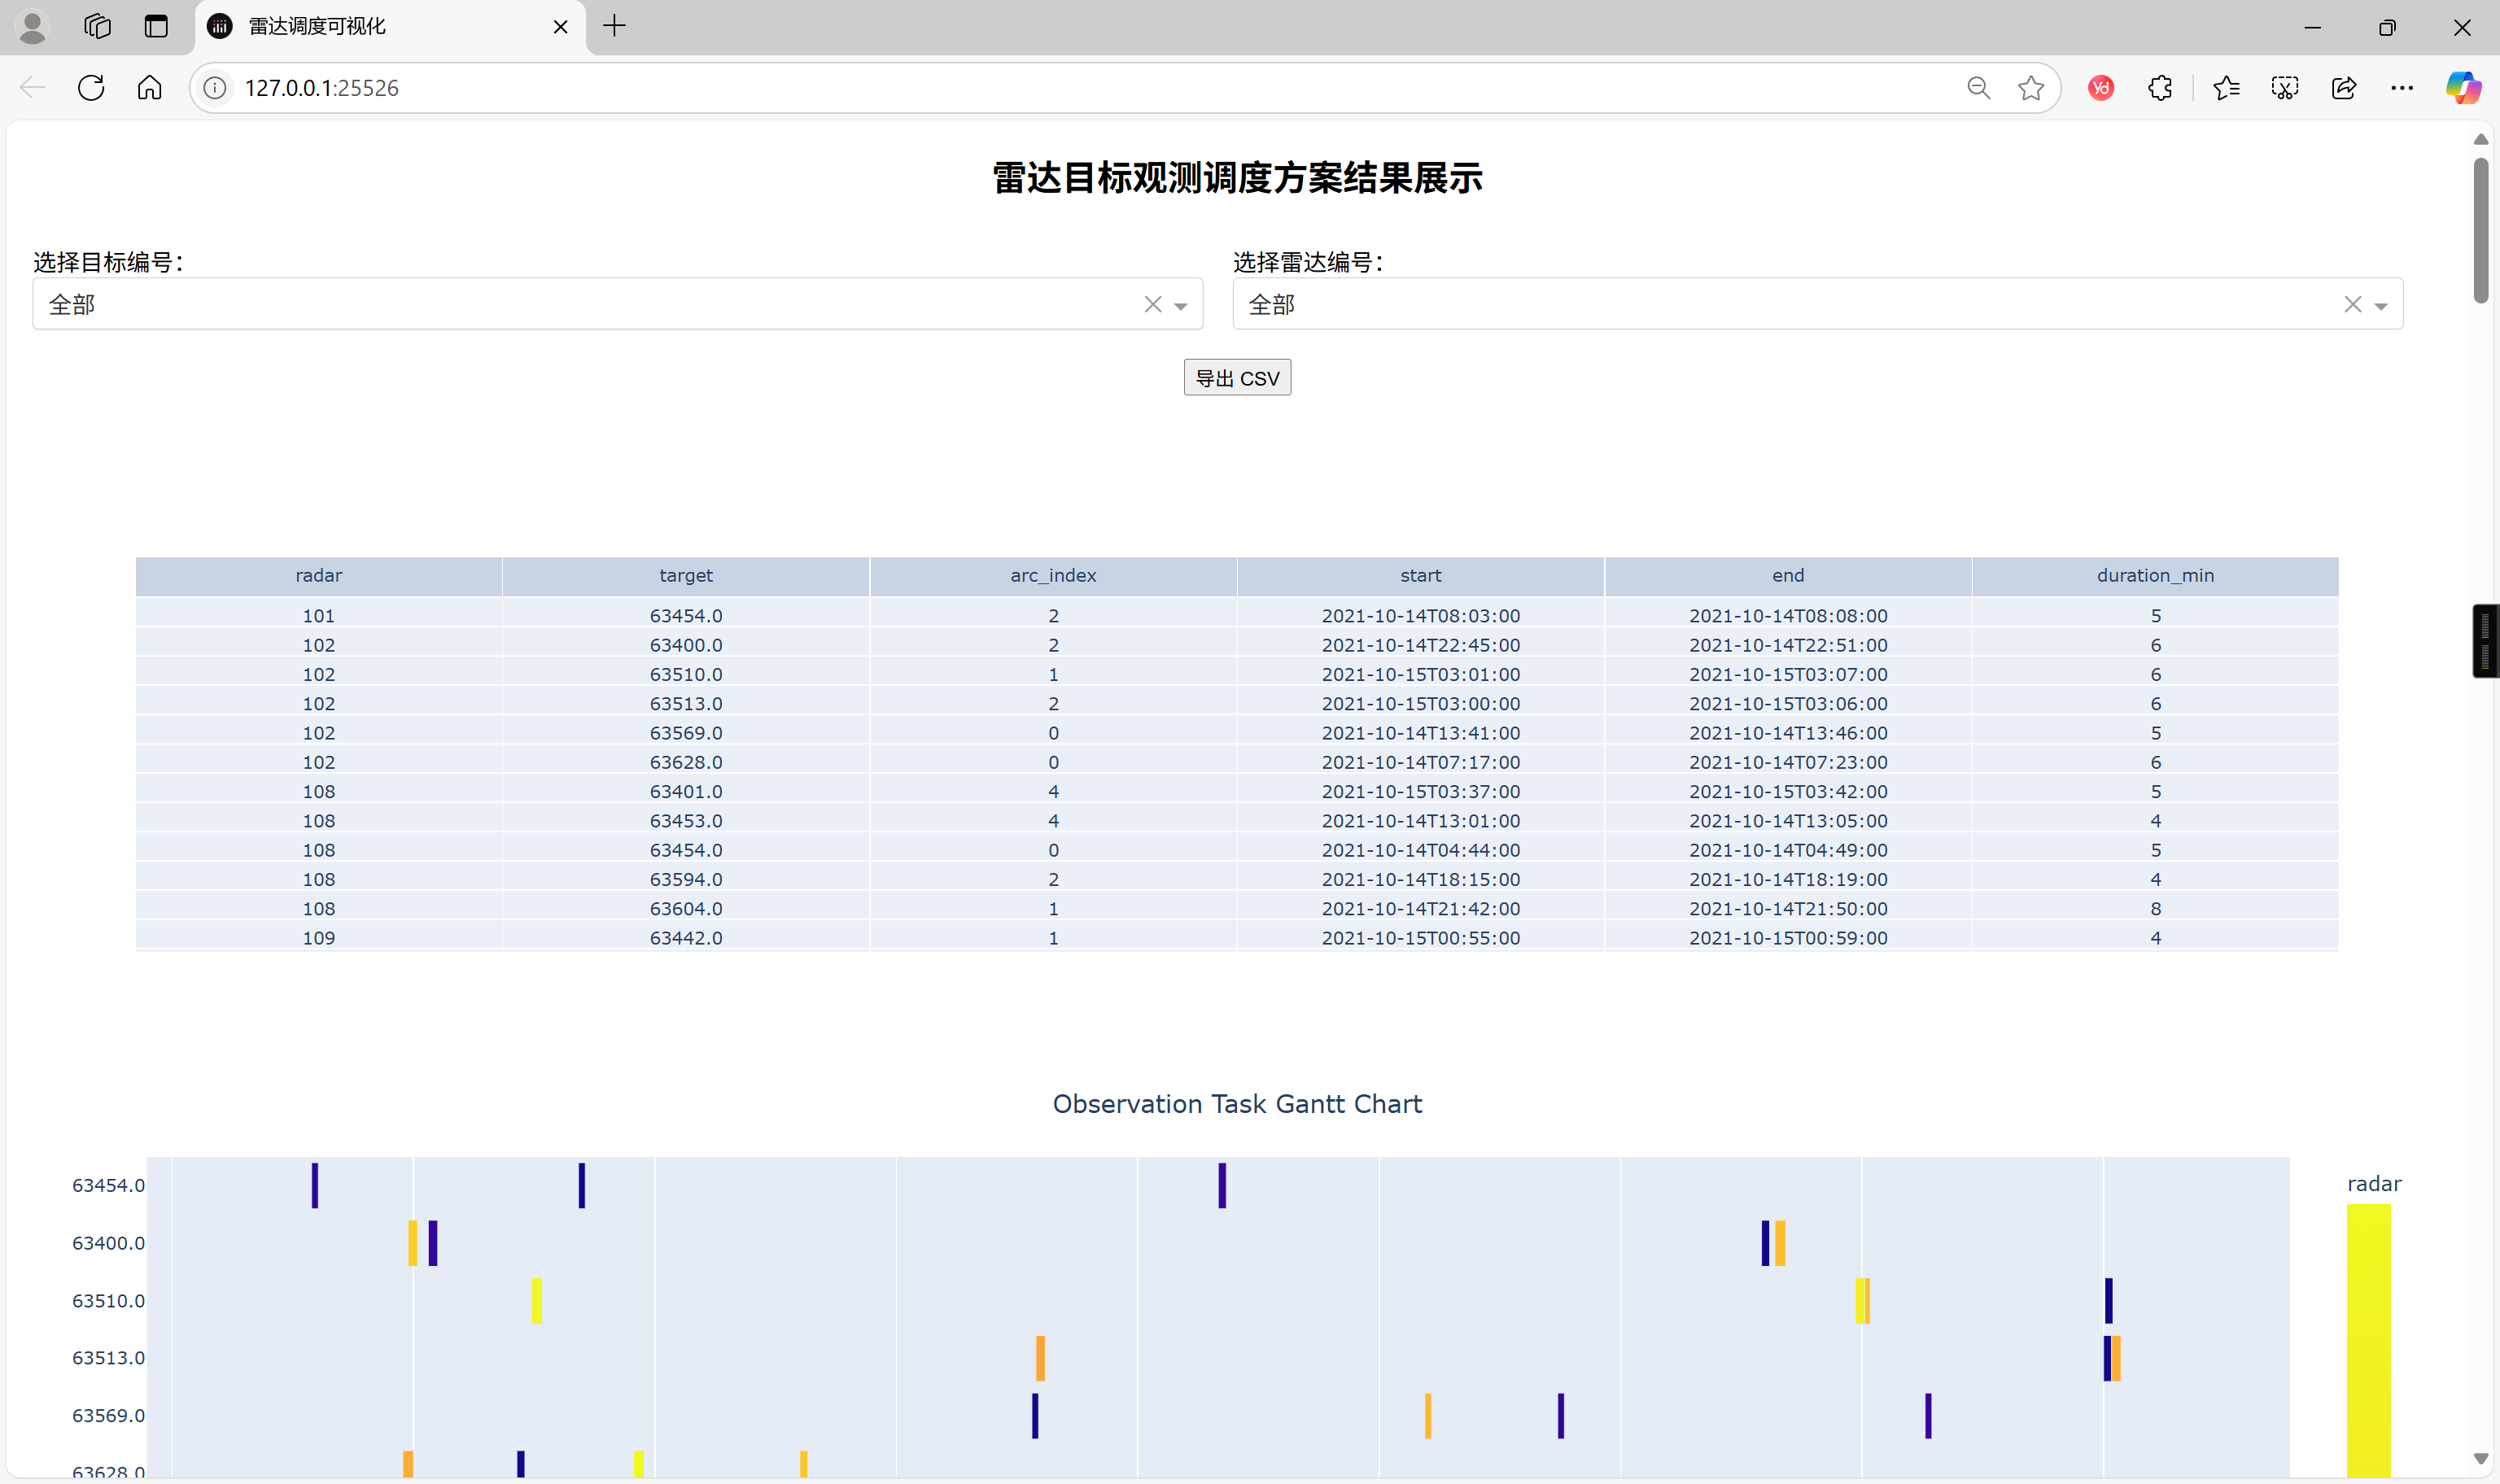
\includegraphics[width=\columnwidth]{figures/网页界面示意.png}
    \caption{网页界面示意}
    \label{figure:网页界面示意}
\end{figure}

\section{探测任务方案评估}
本节将从以下几个方面对探测任务调度方案进行评估:
\begin{itemize}
    \item {目标覆盖效果}:统计有效观测目标的数量及覆盖率,评估调度方案是否满足任务需求;
    \item {资源利用效率}:通过雷达观测弧段总数评估雷达资源的使用效率;
    \item {优先级响应程度}:按优先级统计各层级目标的覆盖率,验证模型是否合理响应优先级设定;
    \item {计算性能表现}:评估模型求解时间、收敛速度及稳定性。
\end{itemize}

评估结果如\autoref{tab:results_summary}所示。模型在优先保障高权重目标的前提下,仍能兼顾大量中低优先级目标的观测需求,体现了良好的任务协调能力。此外,雷达资源利用较为紧凑,观测弧段总数控制在合理范围内,表明模型具有较高的资源调度效率。
\begin{table}[h]
    \centering
    \caption{探测任务规划求解结果统计}
    \label{tab:results_summary}
    \begin{tabular}{ll}
        \toprule
        \textbf{指标}        & \textbf{数值}      \\
        \midrule
        最终目标值(加权有效观测目标数)   & 1476.0           \\
        最终雷达观测弧段总数         & 654.0            \\
        总目标数量              & 193              \\
        有效观测目标数量           & 188              \\
        覆盖率                & 97.41\%          \\
        高优先级目标覆盖率(优先级 > 8) & 63/65 → 96.92\%  \\
        中优先级目标覆盖率(优先级 > 6) & 96/99 → 96.97\%  \\
        低优先级目标覆盖率          & 29/29 → 100.00\% \\
        \bottomrule
    \end{tabular}
\end{table}

\section{拓展思考}
通过本次“探测任务规划”与前期“近距离观测轨迹规划”的仿真实践,我对航天任务规划问题有了更深入的理解。航天任务规划本质上是一个复杂的资源调度与多目标优化问题,其核心在于如何在有限的时间与设备资源下,最大化任务收益并保障任务可行性。

在任务评估方面,我认为应从以下几个维度开展:

\begin{itemize}
    \item \textbf{任务完成度}:是否满足所有硬性约束(如观测次数、测站数量、时间限制等);
    \item \textbf{资源效率}:是否高效利用了可用资源,避免浪费;
    \item \textbf{优先级响应}:是否按照设定的优先级顺序执行任务;
    \item \textbf{鲁棒性与容错性}:在突发情况下能否快速调整调度方案;
    \item \textbf{可扩展性}:模型是否易于适应更大规模或更多任务场景。
\end{itemize}

未来可进一步引入不确定性因素(如天气干扰、设备故障等),构建更具现实意义的鲁棒调度模型,并探索强化学习等智能算法在任务规划中的应用潜力。

\begin{sidewaystable}[h]
    \centering
    \caption{主要数据结构与符号说明}
    \label{table:主要数据结构与符号说明}
    \begin{tabularx}{\columnwidth}{llXl}
        \toprule
        类别   & 符号/变量                                                  & 含义                                             & 数据类型                       \\
        \midrule
        集合   & $R$ / \texttt{radars}                                  & 雷达编号集合,编号从0开始                                  & \texttt{list[int]}         \\
             & $S$ / \texttt{targets}                                 & 目标编号集合,编号从0开始                                  & \texttt{list[int]}         \\
             & $T$ / \texttt{simDate}                                 & 仿真时间节点序列(UTC)                                  & \texttt{np.ndarray[float]} \\
             & $A_{r,s}$ / \texttt{arc\_indices[(r,s)]}               & 雷达$r$对目标$s$的可用弧段编号集合                           & \texttt{dict[tuple,list]}  \\
        输入数据 & \texttt{sensor\_data}                                  & 测站参数表,包含编号、最大可观测目标数等信息                         & \texttt{DataFrame}         \\
             & \texttt{require\_data}                                 & 各目标观测需求表,包含所需测站数、观测次数、优先级等                     & \texttt{DataFrame}         \\
             & \texttt{usable\_arcs}                                  & 可见弧段原始矩阵(MATLAB格式)                             & \texttt{np.ndarray}        \\
             & \texttt{radar\_target\_vis\_dict}                      & 可见性字典:键为$(r,s)$,值为弧段列表$(start, end, duration)$ & \texttt{dict[tuple,list]}  \\
        模型参数 & $C_r$ / \texttt{radar\_capacities[r]}                  & 雷达$r$的最大同时观测能力                                 & \texttt{np.ndarray[int]}   \\
             & $M_s^{\min}$ / \texttt{required\_stations[s]}          & 目标$s$需被多少个测站观测                                 & \texttt{np.ndarray[int]}   \\
             & $N_s^{\min}$ / \texttt{required\_arc\_count[s]}        & 目标$s$需被观测的有效弧段数量                               & \texttt{np.ndarray[int]}   \\
             & $T_s^{\min}$ / \texttt{required\_observation\_time[s]} & 目标$s$需累计观测时间(分钟)                               & \texttt{np.ndarray[float]} \\
             & $w_s$ / \texttt{priority\_weights[s]}                  & 目标$s$的观测优先级权重                                  & \texttt{np.ndarray[float]} \\
        决策变量 & $x_{r,s,a}$ / \texttt{x[r][s][a]}                      & 布尔变量,表示是否在弧段$a$对目标$s$进行观测                      & \texttt{coptpy.Var}        \\
             & $y_s$ / \texttt{y[s]}                                  & 布尔变量,表示目标$s$是否被有效观测                            & \texttt{coptpy.Var}        \\
        \bottomrule
    \end{tabularx}
\end{sidewaystable}

\begin{sidewaystable}[h]
    \centering
    \caption{部分调度方案摘要(前10项)}
    \label{tab:schedule_summary}
    \begin{tabular}{|c|c|c|c|c|c|}
        \hline
        \textbf{雷达编号} & \textbf{目标编号} & \textbf{弧段索引} & \textbf{开始时间 (UTC)} & \textbf{结束时间 (UTC)} & \textbf{持续时间 (分钟)} \\
        \hline
        101.0         & 63454.0       & 2             & 2021-10-14T08:03:00 & 2021-10-14T08:08:00 & 5.0                \\
        \hline
        102.0         & 63400.0       & 2             & 2021-10-14T22:45:00 & 2021-10-14T22:51:00 & 6.0                \\
        \hline
        102.0         & 63510.0       & 1             & 2021-10-15T03:01:00 & 2021-10-15T03:07:00 & 6.0                \\
        \hline
        102.0         & 63513.0       & 2             & 2021-10-15T03:00:00 & 2021-10-15T03:06:00 & 6.0                \\
        \hline
        102.0         & 63569.0       & 0             & 2021-10-14T13:41:00 & 2021-10-14T13:46:00 & 5.0                \\
        \hline
        102.0         & 63628.0       & 0             & 2021-10-14T07:17:00 & 2021-10-14T07:23:00 & 6.0                \\
        \hline
        108.0         & 63401.0       & 4             & 2021-10-15T03:37:00 & 2021-10-15T03:42:00 & 5.0                \\
        \hline
        108.0         & 63453.0       & 4             & 2021-10-14T13:01:00 & 2021-10-14T13:05:00 & 4.0                \\
        \hline
        108.0         & 63454.0       & 0             & 2021-10-14T04:44:00 & 2021-10-14T04:49:00 & 5.0                \\
        \hline
        108.0         & 63594.0       & 2             & 2021-10-14T18:15:00 & 2021-10-14T18:19:00 & 4.0                \\
        \hline
    \end{tabular}
\end{sidewaystable}
\end{document}